\section{Introduction}
Ever since the development of the Backpropagation
algorithm Supervised Learning has been the most fundamental technique for
training Deep Learning Models. This is not surprising, as it provides a model with clear domain specific
learning signals, which is the most direct and efficient way of solving a problem
or learning a task, respectively \cite{geron}.

However, the philosophy of developing artificial intelligences using labeled
data has its limits. In order for Machine Learning models, and especially Deep Learning models, 
to learn increasingly complex tasks requires increasingly more (labeled) data.
Obviously, creating millions of labeled examples is both costly and becomes more infeasible
the more complex the underlying task gets.

Because of this, Self-Supervised Learning has received an increased attention from the scientific
community over the last few years. This is because Self-Supervised Learning does not
rely on creating labeled data by hand, e.g. through human annotation, but receives it
from the context of the data. To train a Large-Language Model (LLM) to understand 
written text, for example, words in example sentences are masked or
deleted, respectively. The task of the model is then to predict those missing words.


\begin{figure}[htbp]
	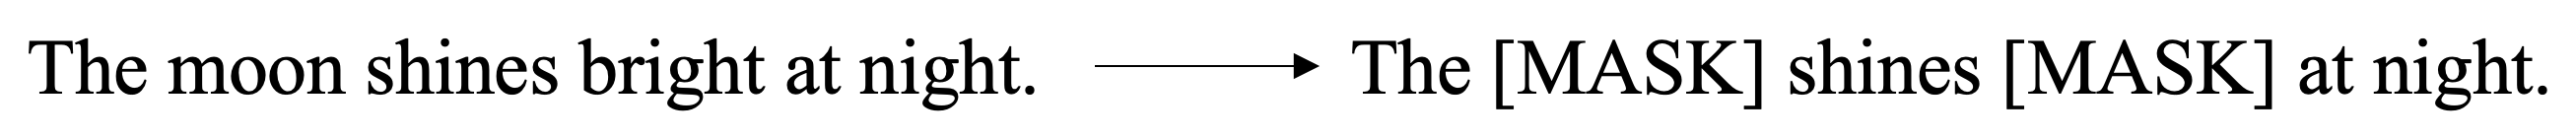
\includegraphics[width=12cm]{language_masking}
	\centering
    \label{language_masking}
	\caption{An example for creating labels out of raw data. Any word in a sentence can
    potentially be masked, which is why training examples (including labels) can be created
    just from the data itself, without any human annotation (adapted from \cite{lecun}).}
\end{figure}

This has three advantages: Firstly, labels do not need to be created by hand, as it is easy
to randomly mask words in a sentence and use them as the targets to predict during training.
Secondly, because there are massive amounts of text available on the internet, a massive amount of training
data can be generated.
And lastly but most importantly, the model learns to write text that represents the world we live in.
This becomes clear with the example seen in Figure \ref{language_masking}.
Here the model would have to predict the words "moon" and "bright" based on the context/words
remaining after masking. In order to do so successfully, the model has to learn that only the moon shines at night, not the
sun, and that if the moon shines, it is usually bright.

The aforementioned example illustrates an important characteristic of Self-Supervised Learning:
It forces the model to learn common sense and the world that we humans live in \cite{lecun}.
In some setting like vision and sound, or even natural language, this is characterized by
creating a representation of the respective input, similar to word embeddings. So for an image
the network might produce a vector that represents the semantic content of that image \cite{wu}\cite{he}\cite{chen},
which is called Representation Learning.

This makes Self-Supervised Learning suitable as a generic pre-training task: If a model
can understand text, images, or sound that reflects the world we live in, then it
can be fine-tuned to various downstream tasks.
A model that has learned to extract the content of an image can be used
to detect cats and dogs with only little fine-tuning, which is significantly simpler than
training a model from scratch.
It follows that for supervised tasks such pre-trained models needs less human annotated examples because they
already understand the data itself.

Up until now only few models have been developed that combine Self-Supervised Learning
of different modalities, most prominently natural language, vision and sound, into one single model.
This by some called "big convergence" \cite{wang} has its foundation in the fact
that concepts of the real world are not bound to a specific modality, but rather
expressed in one.
Continuing the previous example (Figure \ref{language_masking}): The concept of the moon shining at night does not change
when expressed as text, photographed in an image, or spoken using sound.
Therefore, the same concept should always have the same representation regardless of the modality
in which the network receives it.

In order for this to work, a model is required that can process multiple modalities and create
representations for the concepts that are expressed using those modalities, which is called Multimodal
Representation Learning.

\section{Objectives and Research Question}

The research in the master thesis focuses on Multimodal Representation Learning, and will consist of three research parts.

At first, the goal is to construct a Multimodal model based on the paper Data2Vec \cite{baevski}, 
which lays the foundation to combine different modalities into one model.
Because Data2Vec only provides the learning tasks to train one model jointly on text, vision and sound,
the thesis will test different architectures motivated on three other papers, which specifically
address Multimodal Representation Learning, namely VLMo \cite{bao}, BEiT \cite{wang} and FLAVA \cite{singh}.

Joined with this effort, the thesis will evaluate the effect
of the model size on the quality of the representations, as there has been a trend to 
scale language and vision models to billions of parameters, making it infeasible to train
them outside big corporations. Therefore, the thesis will test which procedure provides the best trade-off between size,
training speed and performance.
Regarding performance, it will be interesting if a pre-trained multimodal model is able to 
achieve the same performance on downstream tasks (e.g. ImageNet-1k) as an 
unimodal (one that has learned only e.g. image representation) model of the same size would.

The second part or the research will investigate the properties of
representations generated by a multimodal model. This includes a thorough analysis on a modality-invariance
of the representations, so if, for example, the text "The moon shines bright at night"
and a corresponding image of the moon at night will have similar, or even the same, representations.

The last part of the thesis focuses on latent-space arithmetic for Representation Learning.
The goal here is to create representations with which one can perform arithmetic similar to word embeddings.
This includes, for example, creating a representation of an image with a persons face, and creating
a representation of a sentence about sunglasses. If one now adds the representation of the sunglasses to
the representation of the face, and generates text from the resulting representation, then the resulting text
should be about a person wearing sunglasses.

In order for this to be successful, it might be necessary to develop a Multimodal Autoencoder that is both
able to create representations of its input data, and to generate new data from those representations.

In summary, the contributions and research questions of the master thesis are as follows:

\begin{itemize}
	\item Construction of a Multimodal Model based on Data2Vec.
	\item How do smaller models impact Representation Learning?
    \item Do multimodal representations match across modalities?
	\item Does latent-space arithmetic work between representations created from different modalities?
\end{itemize}

\section{Methodology}
The research will start with the selection of appropriate datasets, some of which will be used to
train the multimodal models, while others will be used for fine-tuning the pre-trained models to receive
benchmarks on which the models developed can be compared with others of the scientific community.

At first, the thesis aims to develop a multimodal Data2Vec model, as this is necessary
to examine the properties of the produced representations in the second part of the thesis, and to compare
them with the representations produced by a multimodal Variational Autoencoder.
Another reason behind this order is to first get hands-on experience with Multimodal Representation Learning,
as the examination of a multimodal latent space, using a Variational Autoencoder, has seen considerable less
attention from the scientific community, which induces more risk regarding the success of such a multimodal
Variational Autoencoder.

\section{Solution Ideas}
As may have become apparent in the previous chapters, the development will be based on Data2Vec \cite{baevski}
for the training tasks, and the architecture will be oriented on VLMo \cite{bao}, BEiT \cite{wang} and FLAVA \cite{singh}.
Because all models developed will be multimodal, it is inevitable that the general architecture will be
based on the (Vision \cite{dosovitskiy}) Transformer \cite{vaswani}.

To evaluate the success of the latent-space arithmetic, covered in the last section of the thesis, it is necessary
to develop a model which is not only able to create semantic representation of its inputs, but also able to
produce new samples, namely text, images and sound, from the latent space in which the representations exist.
For this a Variational Autoencoder is suitable, which is usually trained as an unimodal model, but will be
adapted as a multimodal model in this thesis.

\section{Preliminary Structure}

\begin{enumerate}
    \item Introduction
        \begin{enumerate}
            \item Motivation
            \item Research Questions and Contributions
            \item Structure
        \end{enumerate}
    \item Representation Learning
        \begin{enumerate}
            \item Latent-Space Arithmetic
        \end{enumerate}
    \item Multimodal Learning
        \begin{enumerate}
            \item Pre-training Tasks and Requirements
            \item Data2Vec
            \item VLMo
            \item BEiT
            \item FLAVA
            \item Variational Autoencoders
        \end{enumerate}
    \item Methodology
        \begin{enumerate}
            \item Relevance of Uncurated Datasets
            \item Datasets
            \item Metrics and Benchmarks
        \end{enumerate}
    \item Research
        \begin{enumerate}
            \item Experiments on Multimodal Data2Vec
            \item Study on Multimodal Latent Space
            \item Latent-Space Arithmetic with Multimodal Variational Autoencoders
        \end{enumerate}
    \item Outlook
    \item Conclusion
\end{enumerate}

\section{Timeline}